\section{Theorie}
\label{sec:Theorie}
\subsection{Grundlagen und Doppler-Effekt}
Um das Impuls-Echo-Verfahren zu verstehen, ist eine modellhafte Betrachtung des \textit{Doppler-Effekts} sinnvoll.
Der \textit{Doppler-Effekt} beschreibt eine Frequenzverschiebung von Wellen, deren Sender sich zum Zeitpunkt der Wellenerzeugung relativ zum Empfänger bewegen.
Dieser Effekt basiert unter anderem auf dem Huygens'schen Prinzip, nach dem jeder Punkt einer Wellenfront stets Erzeuger neuer Kreis- beziehungsweise Kugelwellen ist.
Durch dieses Prinzip werden Reflexionen von Wellen beschrieben. Die reflektierten Wellen verhalten sich dann so, als wäre das reflektierende Objekt der Erzeuger der Wellen.
Die geometrische Bedeutung dieser beiden Phänomene ist in den Abbildungen \ref{fig:doppler} und \ref{fig:huygen} zu sehen.

\begin{figure}
    \centering
    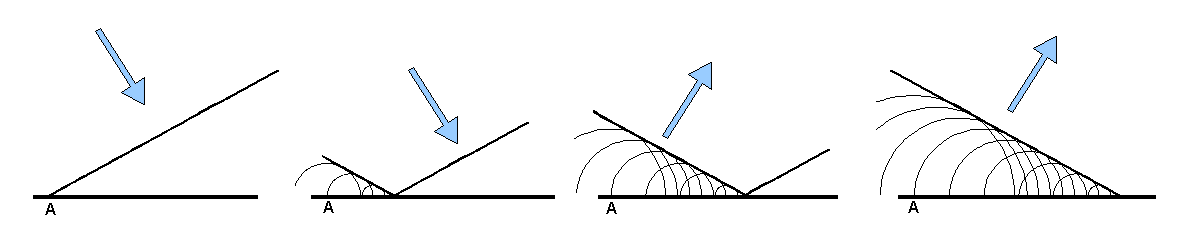
\includegraphics[width=\textwidth]{media/Reflexion_im_Wellenmodell.png}
    \caption{\textit{Huygens'sches Prinzip}: Reflexion im Wellenmodell. \cite{huygens}}
    \label{fig:huygen}
\end{figure}

\begin{figure}
    \centering
    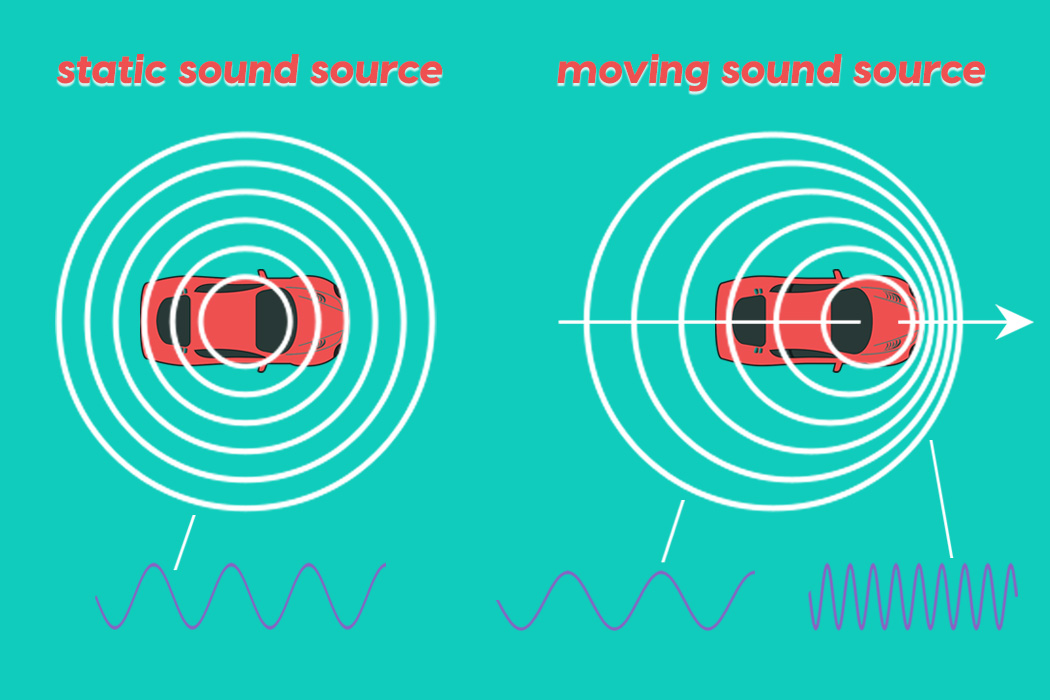
\includegraphics[width=.6\linewidth]{media/doppler-effect-header.jpg}
    \caption{\textit{Doppler-Effekt}: Kompression und Expansion der Wellendichte bei bewegten Erzeugern. \cite{doppler}}
    \label{fig:doppler}
\end{figure}

Das in diesem Versuch angewendete Verfahren nutzt aus, dass eine Reflexion das Verhältnis zwischen Sender und Empfänger umkehrt und der Wellenerzeuger gleichzeitig ein Empfänger sein kann.

\begin{figure}
    \centering
    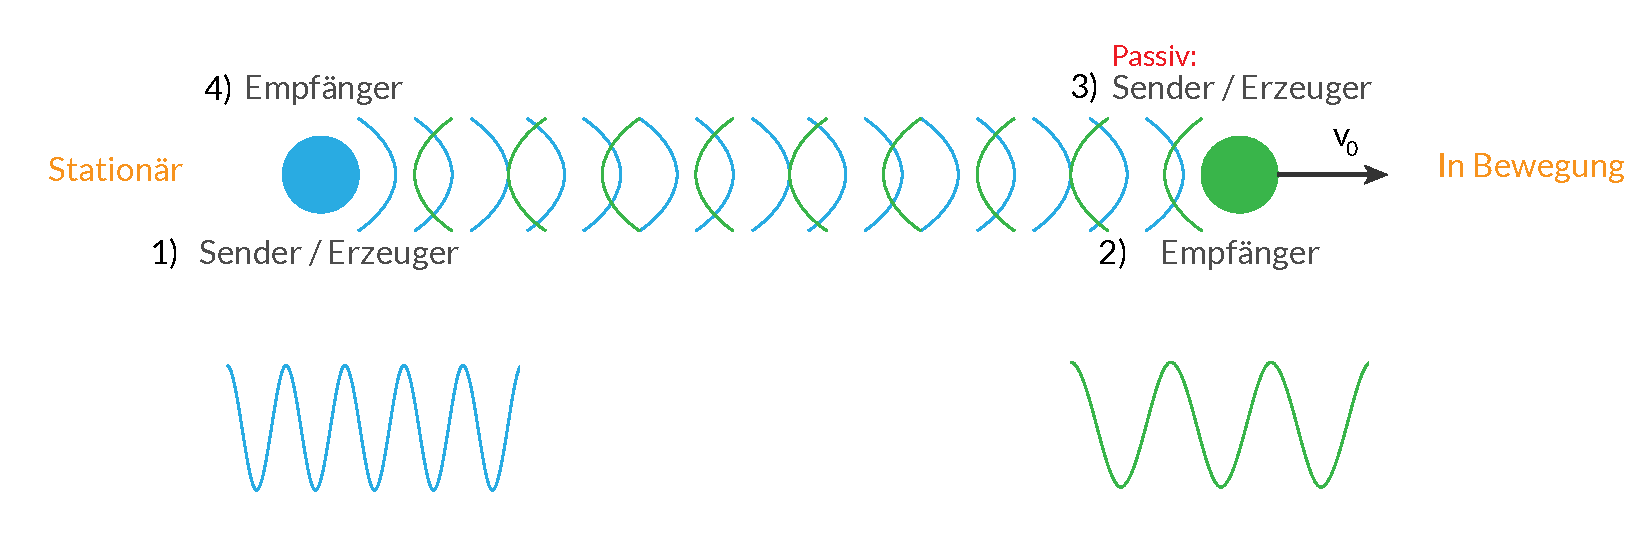
\includegraphics[width=.95\textwidth]{media/doppler_SE.pdf}
    \caption{\textit{Doppler-Effekt}: Reflexion an bewegten Objekten; Erzeuger ist auch Empfänger.}
    \label{fig:se}
\end{figure}

Mathematisch werden zwei Perspektiven beschrieben. Befindet sich der \textit{Sender in Ruhe}, bewegt sich die \textit{Quelle} entweder auf den \textit{Sender} zu, oder entfernt sich.
Im ersten Fall wird die Frequenz \textit{kleiner} und verschiebt sich zu $\nu_{kl}$. Im zweiten Fall verschiebt sie sich zur größeren Frequenz $\nu_{gr}$

\begin{equation*}
    \nu_{kl/gr} = \frac{\nu_0}{1 \mp \frac{v}{c}} \:.
\end{equation*}

Hierbei ist $v$ die Geschwindigkeit des bewegten Objekts und $\nu_0$ die anfängliche Senderfrequenz.

Aus der anderen Perspektive ist der \textit{Empfänger in Ruhe}. Die \textit{Quelle} bewegt sich also entweder auf den Empfänger zu ($\nu_h$), oder von ihm weg, wodurch sich eine niedrigere
Frequenz $\nu_n$ ergibt

\begin{equation*}
    \nu_{h/n} = \nu_0 (1 \pm \frac{v}{c}) \:.
\end{equation*}

\subsection{Winkelabhängigkeit des Doppler-Effekts}
Die beispielhafte Abbildung \ref{fig:doppler} mit dem Auto als Sender zeigt, dass die größten Frequenzunterschiede beobachtet werden, wenn direkt vor oder hinter dem Objekt,
also entlang der Fahrtrichtung gemessen wird. Die im 90°-Winkel zur Fahrtrichtung abgegebenen Schallwellen weisen keine Frequenzverschiebung auf. Der Doppler-Effekt ist also winkelabhängig und wird
durch den Cosinus beschrieben

\begin{equation*}
    \Delta \nu = \nu_0 \frac{v}{c}(\cos{\alpha} + \cos{\beta}) \:.
\end{equation*}

Hier sind die Winkel $\alpha$ und $\beta$ die Winkel zwischen der Geschwindigkeitsrichtung und der Wellennormalen der einfallenden beziehungsweise ausgehenden Welle.
Eine Besonderheit des \textit{Impuls-Echo-Verfahren} ist, dass die Winkel der Strahlengänge durch einen Prisma normiert sind. Dadurch sind die Winkel identisch ($\alpha = \beta$).
Die Gleichung vereinfacht sich zu 

\begin{equation}
    \Delta \nu = 2 \nu_0 \frac{v}{c} \cos{\alpha} \:.
    \label{eqn:doppler}
\end{equation}

\begin{figure}
    \centering
    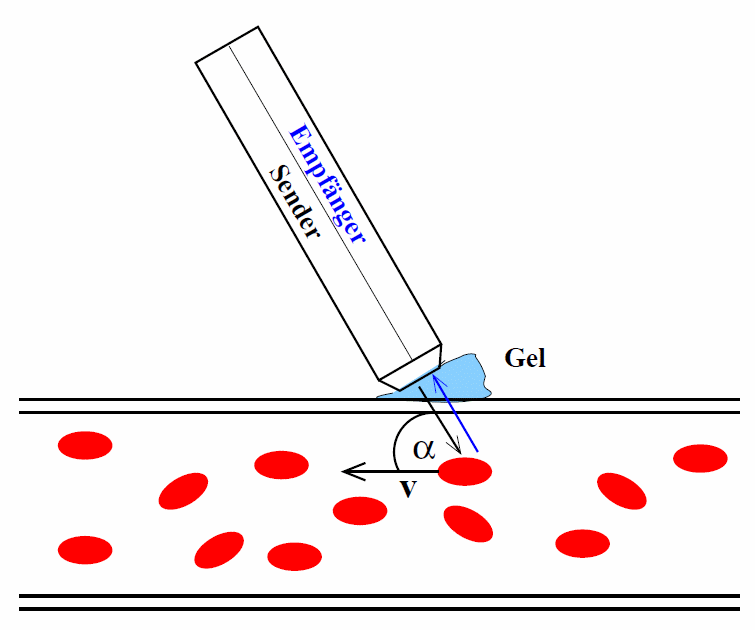
\includegraphics[width=.5\textwidth]{media/echo-impuls-verfahren.png}
    \caption{\textit{Echo-Impuls-Verfahren}. \cite{Versuchsanleitung}}
    \label{fig:eiv}
\end{figure}

\subsection{Erzeugung und Detektion von Ultraschall-Wellen}
Es gibt Festkörper, die ihre Dichte und ihr Volumen ändern, wenn ein elektrisches Feld angelegt wird. Dabei ist die Volumenänderung abhängig von der Stärke des Feldes.
Dieser Effekt, auch \textit{reziproker piezo-elektrischer Effekt} genannt, wird genutzt, um Ultraschall zu erzeugen. Sogenannte \textit{Piezo-Kristalle} werden an eine Wechselspannung angeschlossen und
so in Schwingung versetzt. Es werden Piezo-Kristalle mit Eigenfrequenzen im Ultraschall-Bereich verwendet, um den verstärkenden Effekt der Resonanz zu nutzen.

Umgekehrt können die Kristalle auch als Detektoren von Ultraschall-Wellen dienen. Wird ein Kristall von Ultraschall getroffen, sorgt der lokale Druckunterschied für Schwingungen
und Dichteunterschiede innerhalb des Kristalls. Der Festkörper baut entsprechend dieser Druckunterschiede ein elektrisches Feld auf, dessen Änderung gemessen werden kann. Dies ist der ursprüngliche \textit{piezo-elektrische Effekt}.
Somit kann ein Piezo-Kristall sowohl Sender als auch Empfänger von Ultraschall-Wellen sein (s. Abb. \ref{fig:eiv}), was in dem \textit{Echo-Impuls-Verfahren} auch genutzt wird.

\subsection{Ströumungsprofil und Reynoldszahl}
Das Strömungsprofil einer Röhre mit Radius $R$ ist gegeben \cite{Fluidik} durch
\begin{equation}
    v(r)=v_\text{max}\cdot (1-\frac{r}{R})^{\sfrac{1}{n}}\,,
    \label{eqn:Geschwindigkeit}
\end{equation}
wobei $r$ den Abstand zur Symmetrieachse des Rohrs angibt (also immer $r>0$).
Ist die Strömung laminar (Reynoldszahl kleiner als etwa 2000), ist die Geschwindigkeitskurve parabelförmig, also $n=2$.
$n$ ist schwach von der Reynoldszahl abhängig; außerdem hat die Rauheit der Rohrinnenwand Einfluss auf die Größe der Zahl. 
Für eine sehr große Reynoldszahl $>\num{2e6}$ konvergiert der invertierte Exponent $n$ gegen $n=10$. 

Die Reynoldszahl einer Röhre berechnet sich über 
\begin{equation}
    Re=\frac{\rho v d}{\eta}\,,
\end{equation}
mit der Dichte $\rho$, der mittleren Geschwindigkeit $v$, der charakteristischen Länge $d$, die bei Rohren auf den Durchmesser festgelegt ist, 
sowie der dynamischen Viskosität $\eta$. 
Übersteigt die Reynoldszahl die kritische Reynoldszahl von etwa $2000$, ist die Strömung nicht mehr laminar, sondern turbulent. 